\documentclass[Journal,letterpaper,InsideFigs,NoLists,NoLineNumbers]{ascelike-new}
\WarningFilter{caption}{Unknown document class}
\usepackage[utf8]{inputenc}
\usepackage[T1]{fontenc}
\usepackage{lmodern}
\usepackage{graphicx}
\usepackage[style=base,figurename=Fig.,labelfont=bf,labelsep=period]{caption}
\usepackage{amsmath}
\usepackage{newtxtext,newtxmath}
\usepackage[colorlinks=true,citecolor=red,linkcolor=black]{hyperref}
\usepackage{bm,textcomp,url}
\urlstyle{same}
\graphicspath{{figs/}}
\NameTag{Anticona, \today}
\renewcommand{\thefigure}{S\arabic{figure}}
\renewcommand{\thetable}{S\arabic{table}}
\begin{document}
\title{Supplemental Materials\\[0.5ex] HiBER: Hierarchical Bounded Strength Envelopes for Rockfill and Mine Waste Rock}
\author[1]{Wilson A. Anticona}
\affil[1]{\textbf{[ASCE grade, affiliation, and e-mail to be completed]}}
\maketitle
\noindent This file contains Figs.~S1--S5, Tables~S1--S6, and a worked example of the update, cited in the paper. Equation and table numbers without the prefix S refer to the paper.

\begin{figure}[htbp]
\centering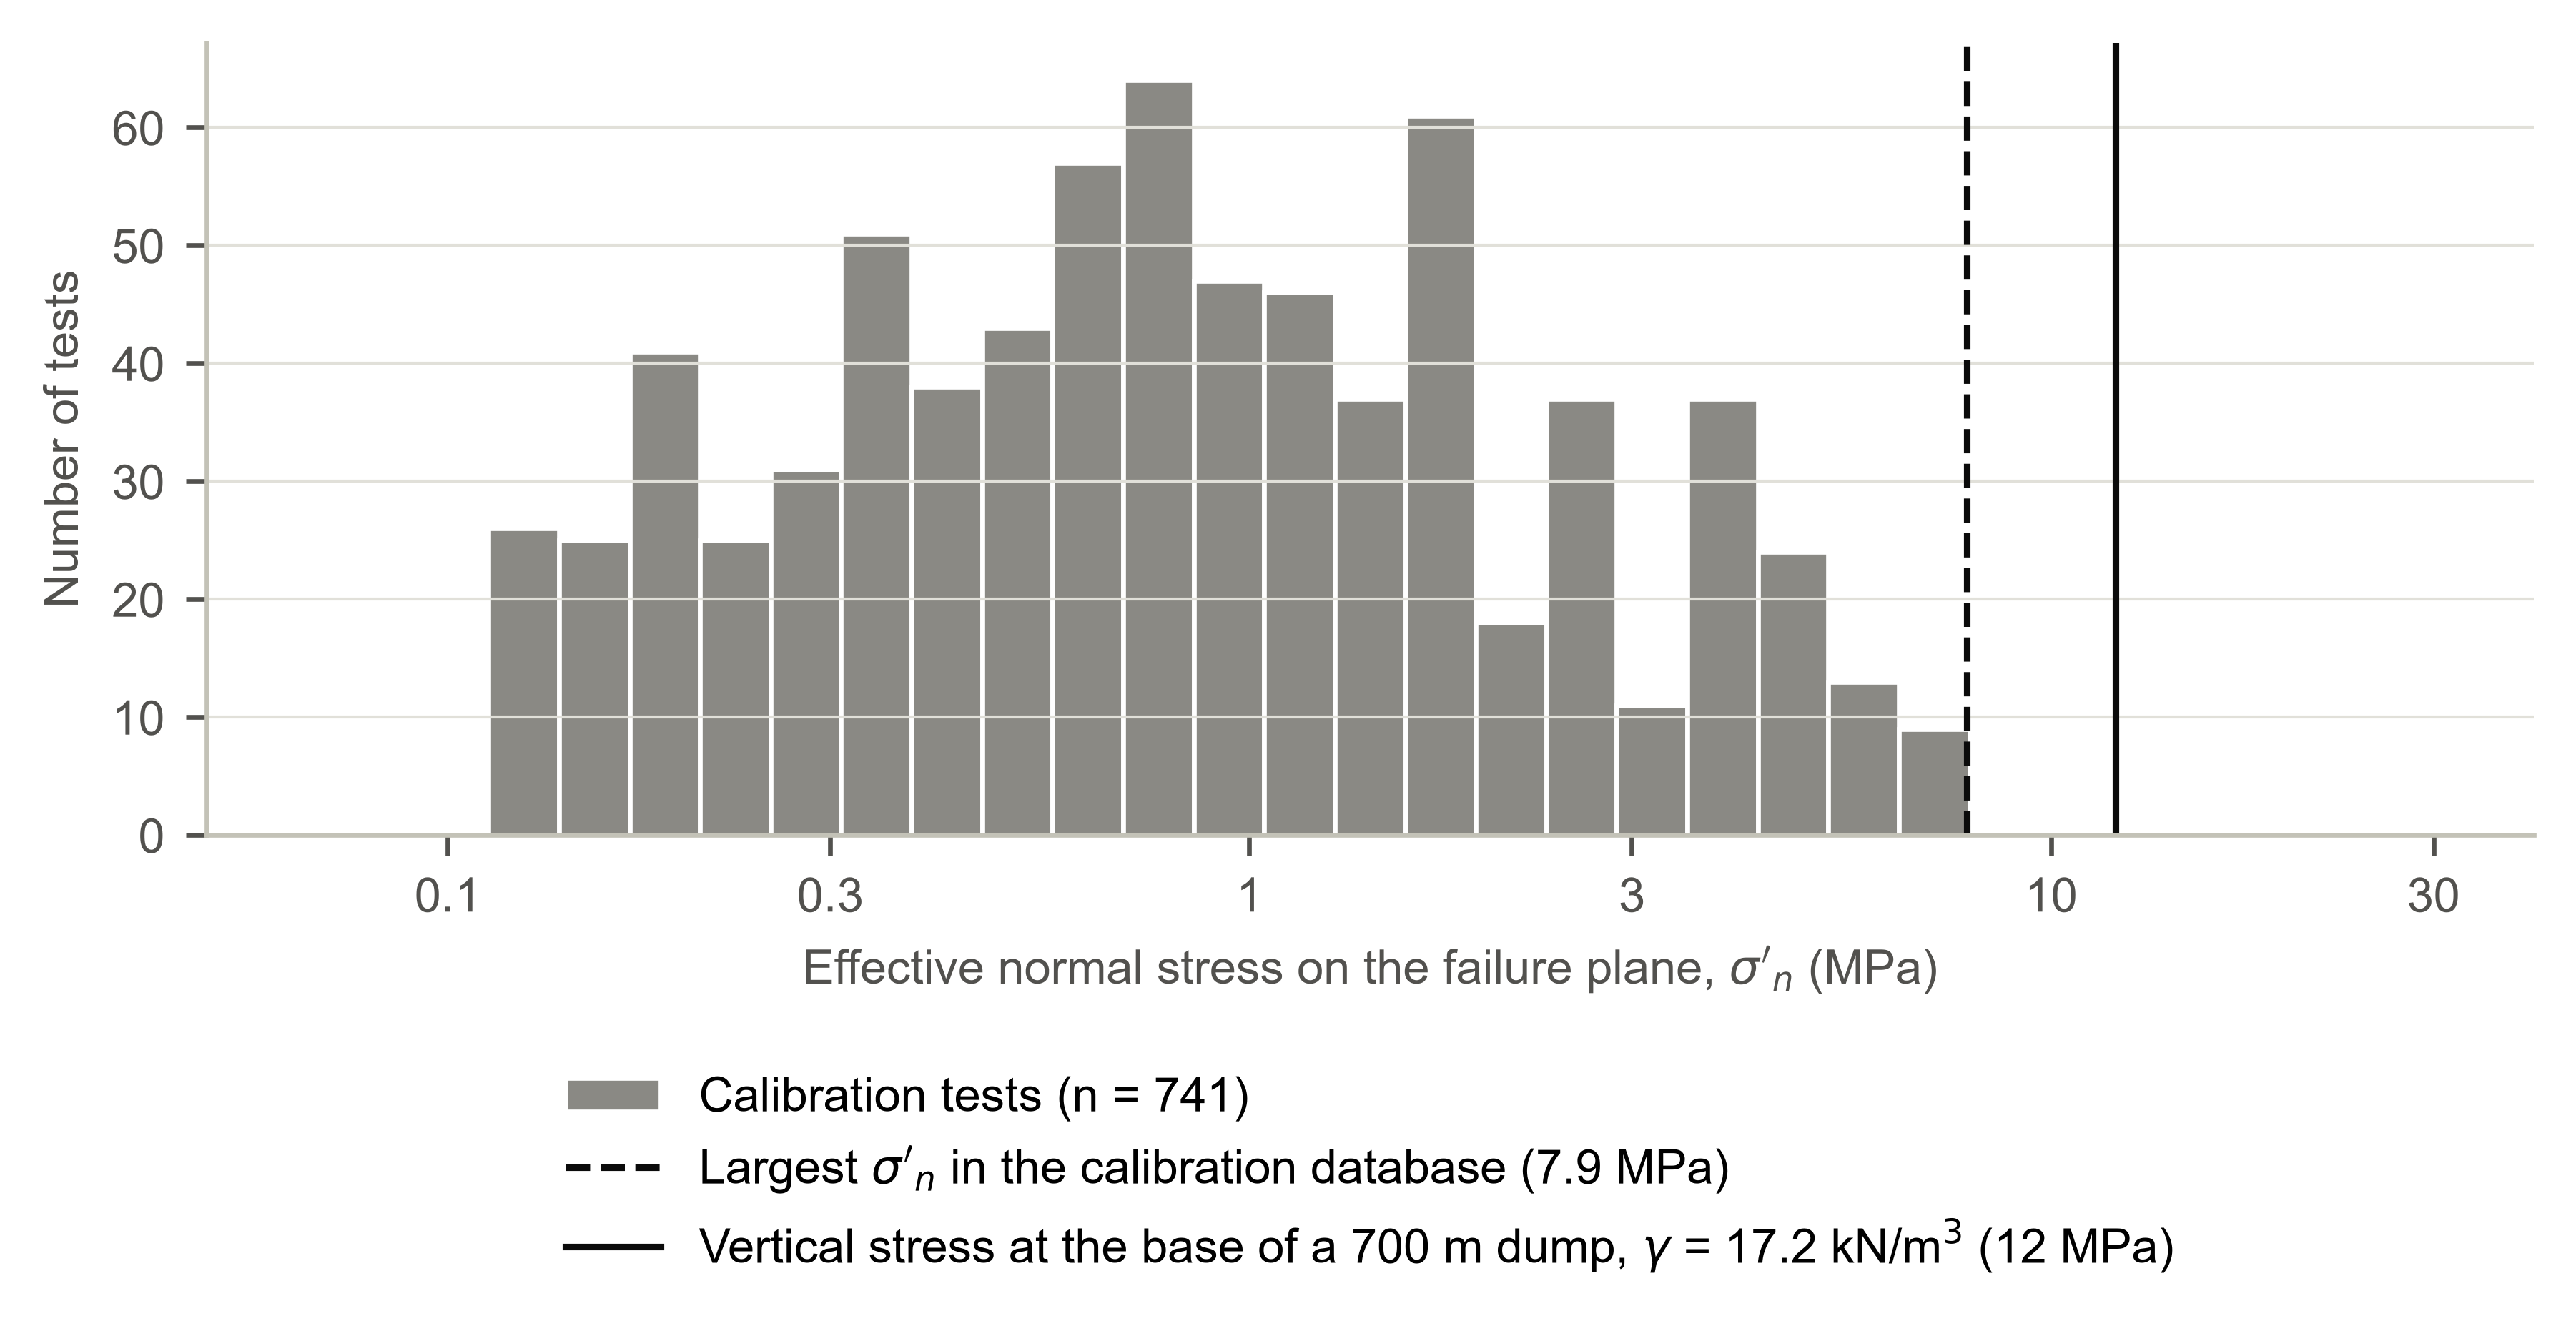
\includegraphics[width=6.0in]{FigS1_stress_coverage.png}
\caption{Distribution of effective normal stress on the failure plane in the calibration database (741 tests).}
\end{figure}
\begin{figure}[htbp]
\centering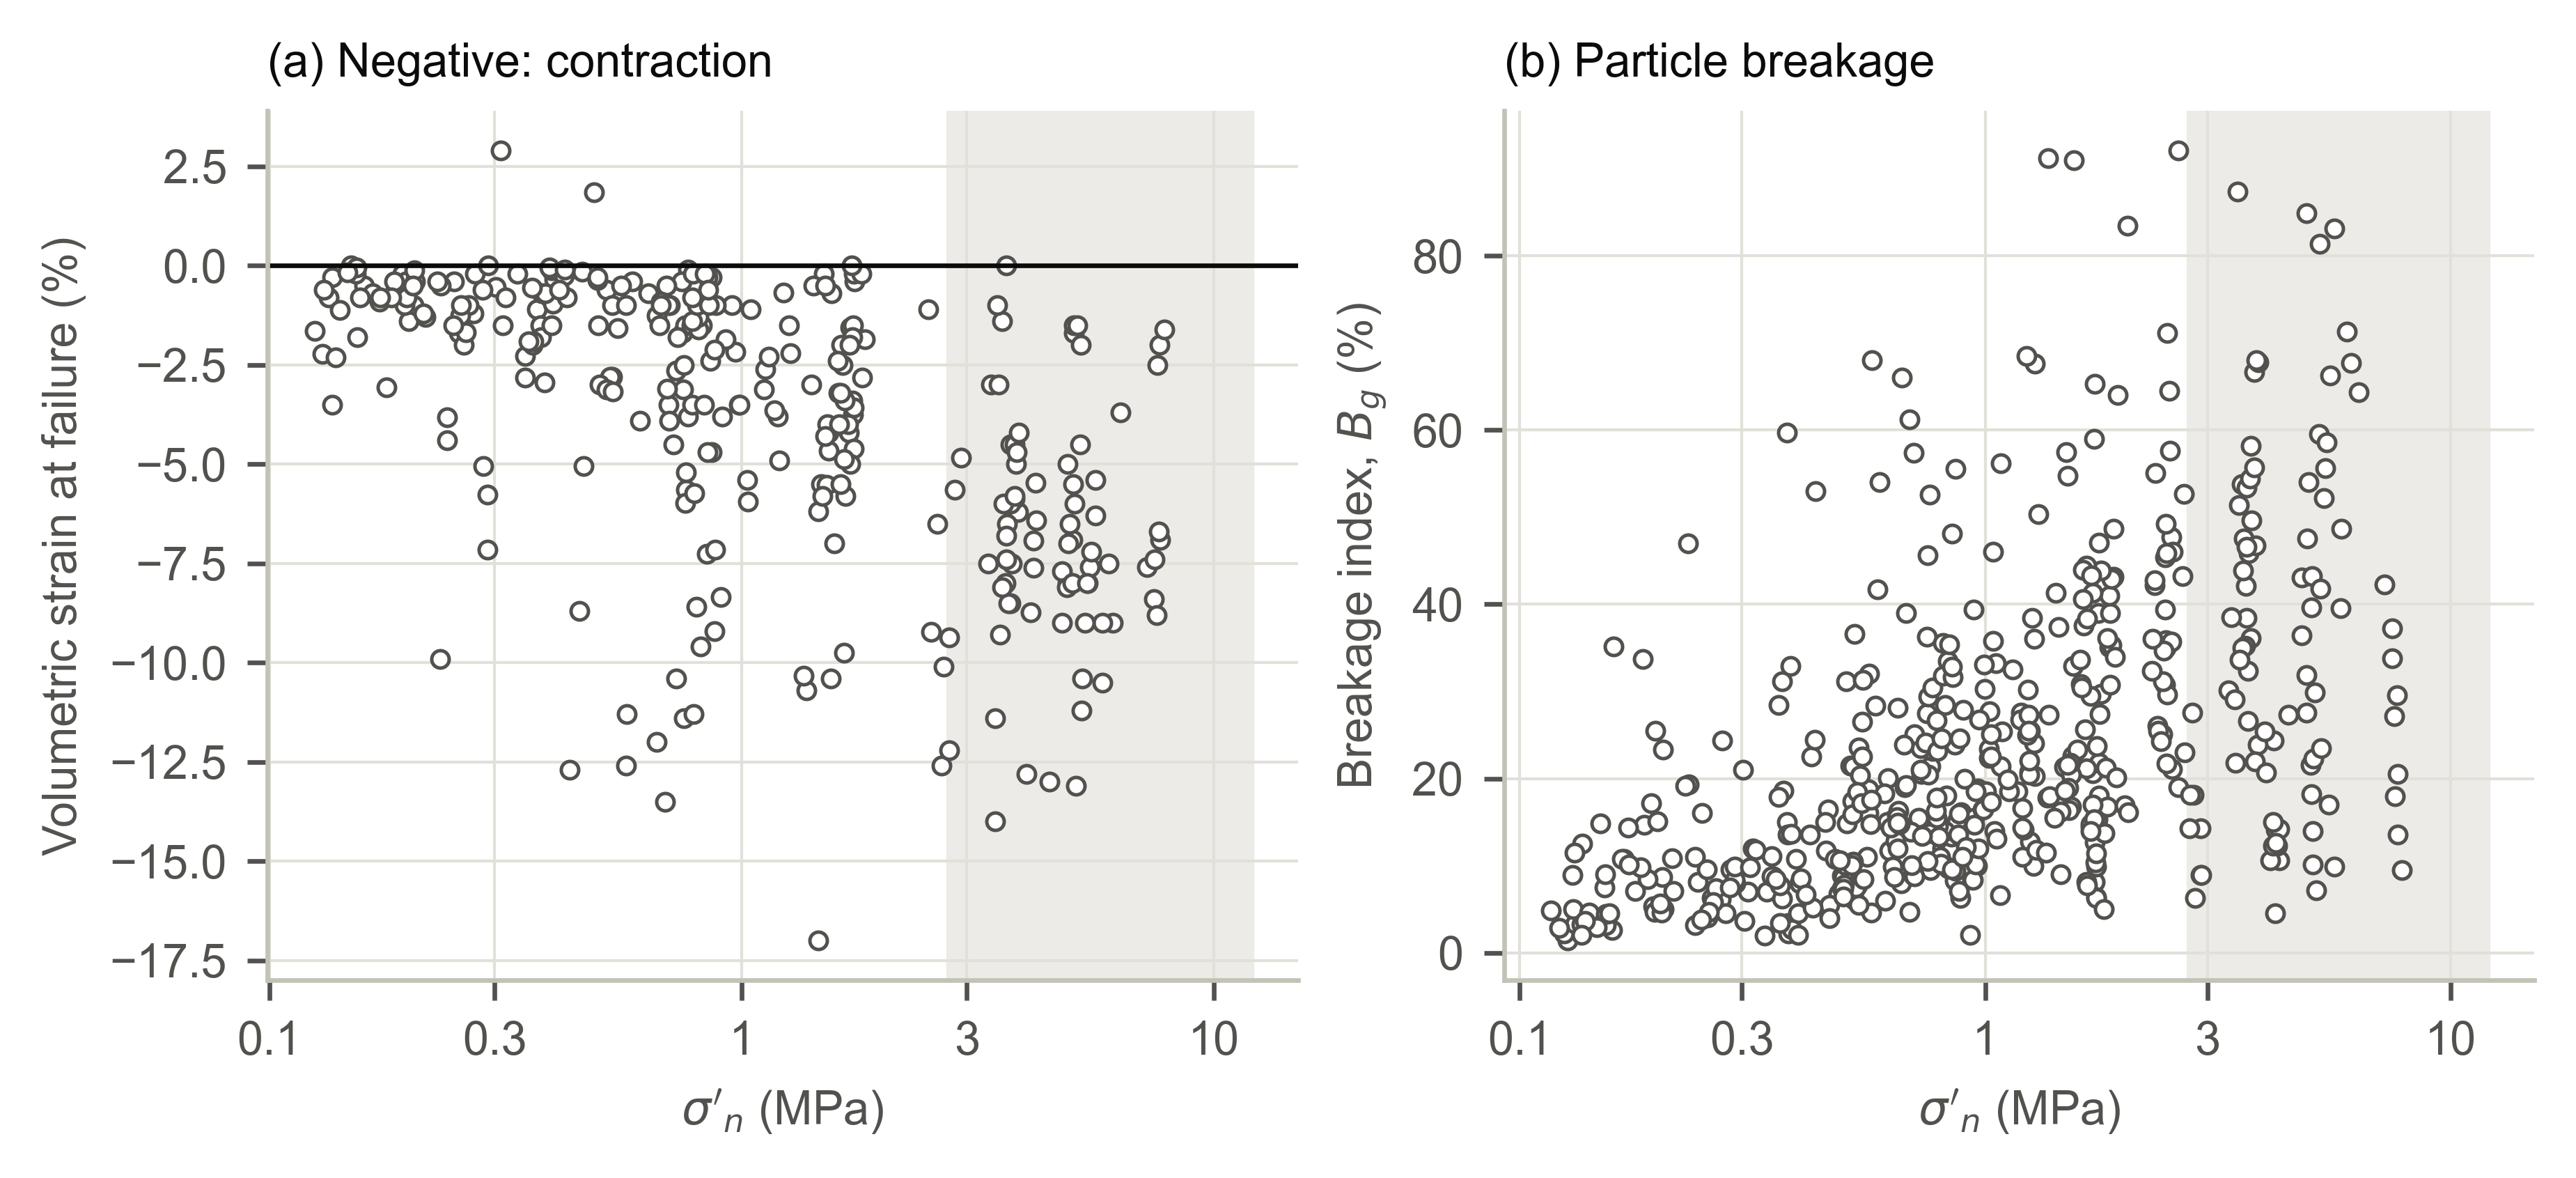
\includegraphics[width=6.0in]{FigS2_volumetric_breakage.png}
\caption{Net volumetric strain at the maximum deviator (negative: contraction) and breakage index of Marsal (1973) versus $\sigma'_n$ in the calibration database. Reported breakage indices above 100\%, impossible by definition, were excluded (4 tests). Above 1.5 MPa the residuals of HiBER increased with the volumetric compression (Spearman $\rho$ = 0.38, n = 122) and, above 2.75 MPa, with the breakage index ($\rho$ = 0.24, n = 91).}
\end{figure}
\begin{figure}[htbp]
\centering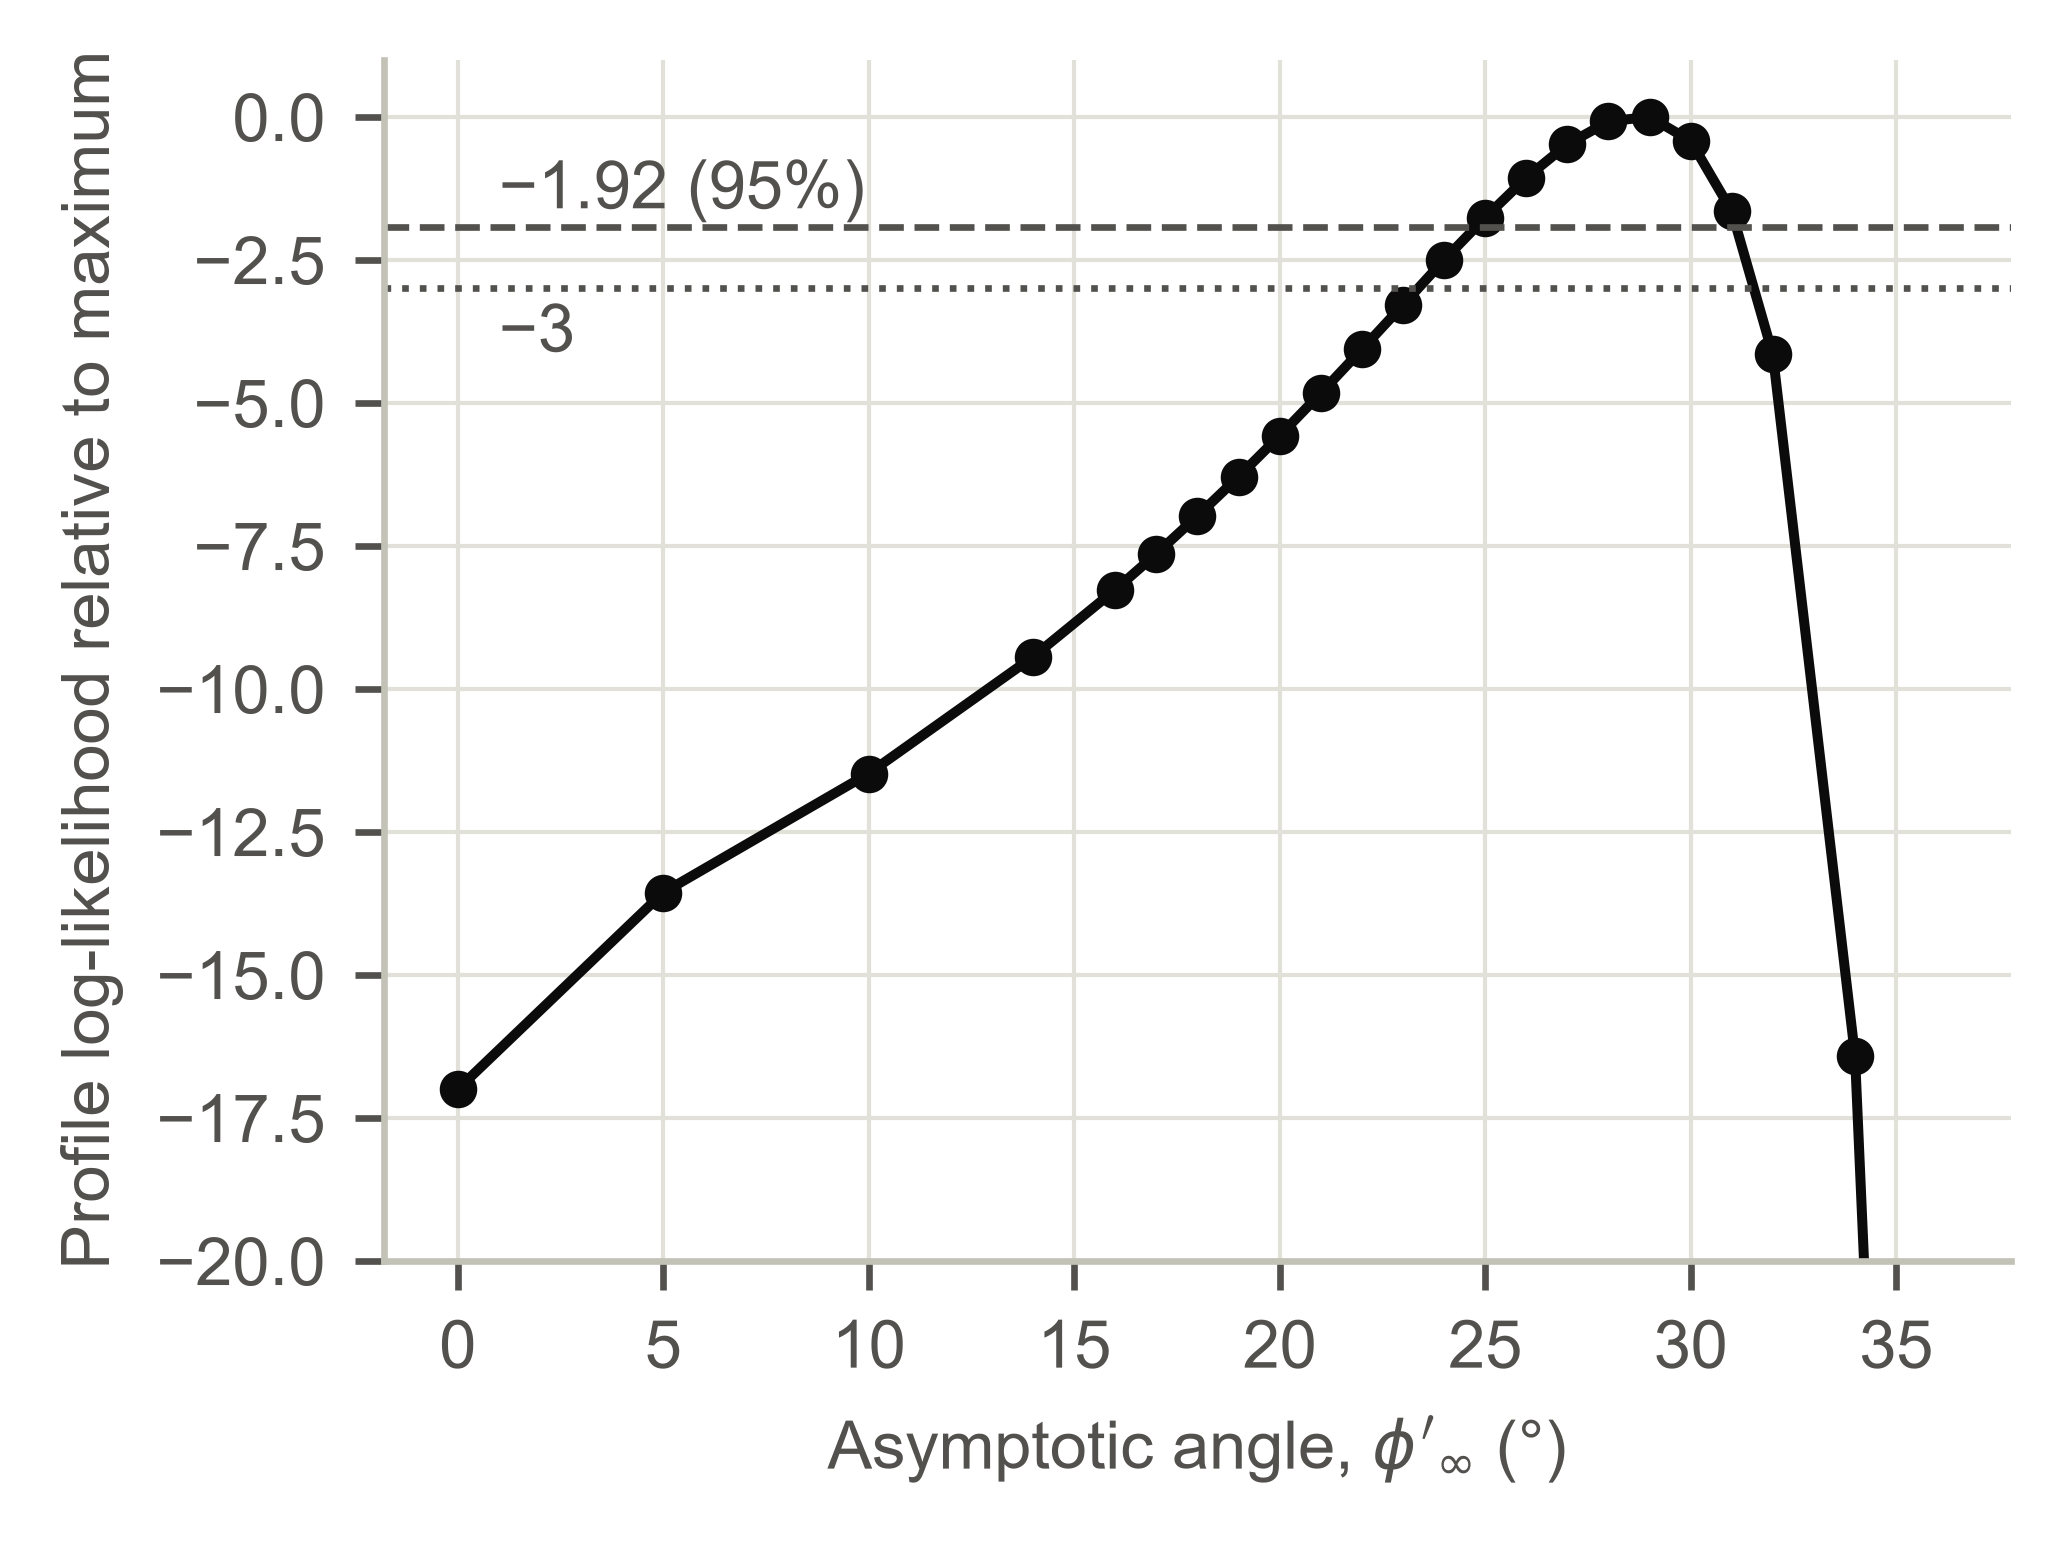
\includegraphics[width=4.0in]{FigS3_profile_likelihood.png}
\caption{Profile of the observed-data log-likelihood (censoring and truncation included) of the asymptotic angle $\phi'_\infty$ relative to its maximum (797.48); at each angle $\zeta_0$, the fixed effects, and the variance parameters were refitted. $\phi'_\infty$ = 0 is the form without an asymptote (approximate: maximum over two values of $\zeta_0$). Dashed: 1.92 units (approximate 95\% interval); dotted: 3 units. First-order approximation; see Table S3.}
\end{figure}
\begin{figure}[htbp]
\centering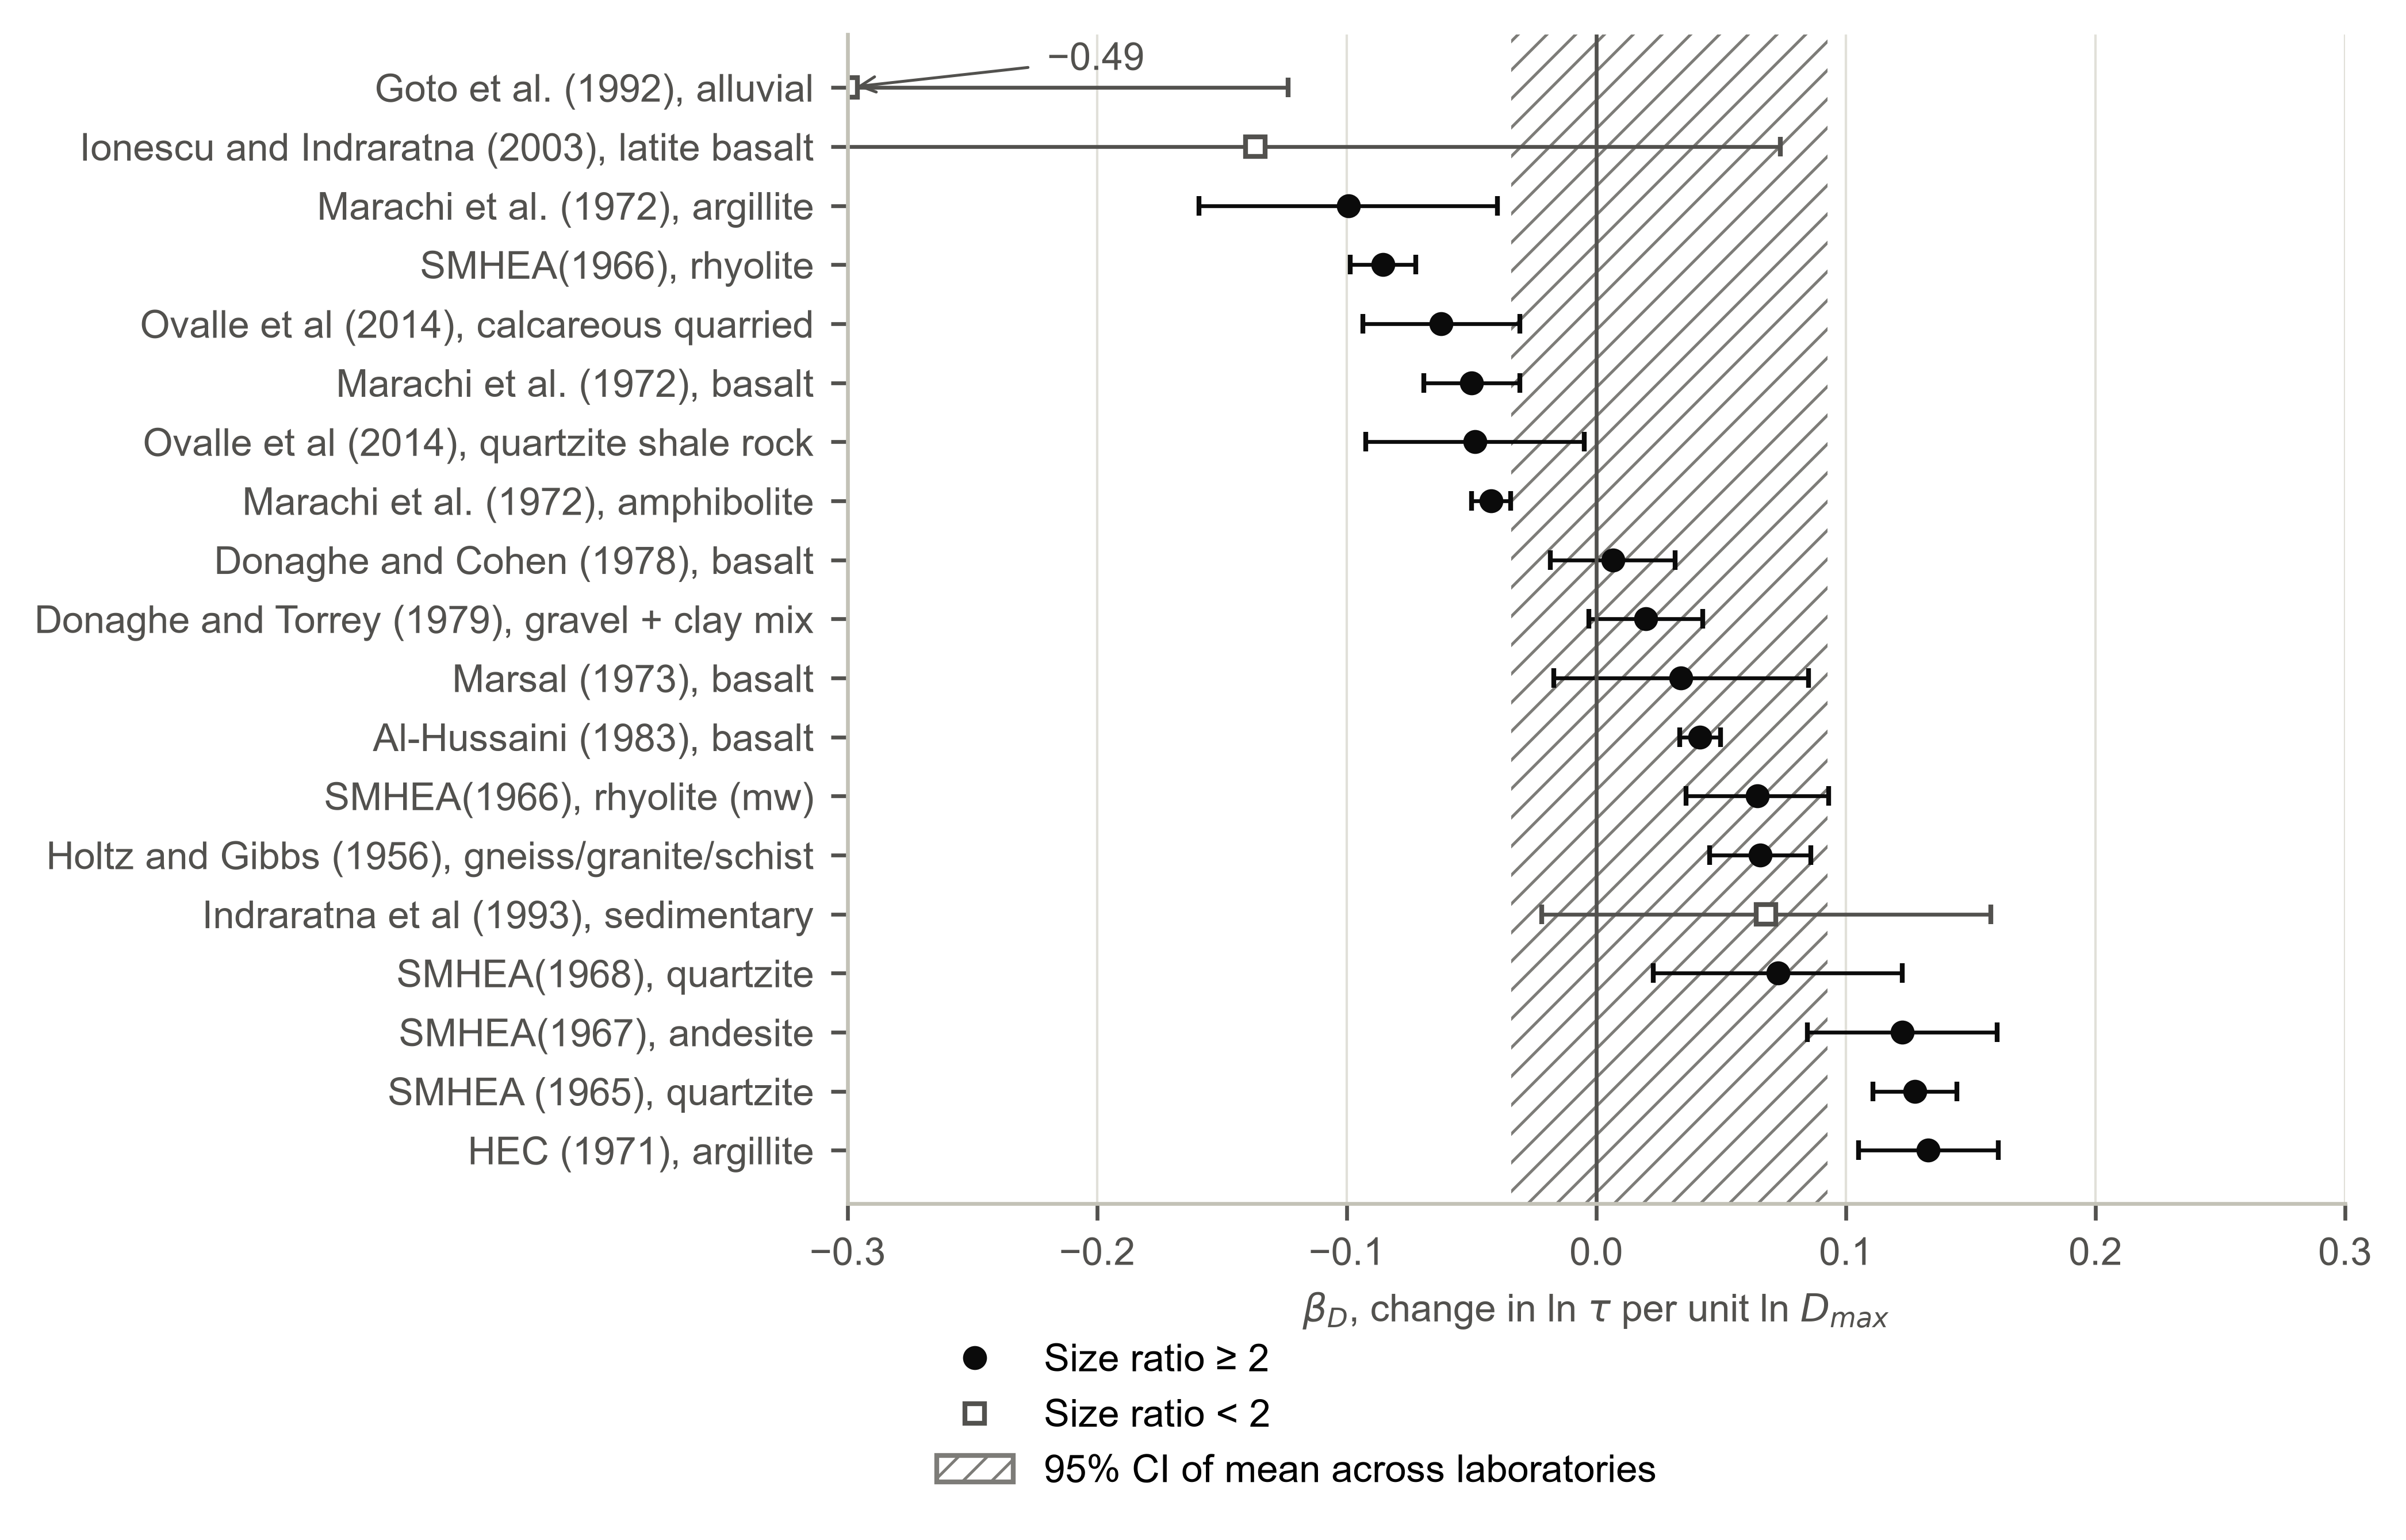
\includegraphics[width=5.6in]{FigS4_size_effect.png}
\caption{Within-material specimen-size coefficient $\beta_D$ by laboratory (bars: 95\% confidence intervals; set intercepts adjusted for void ratio). Hatched band: Knapp--Hartung 95\% confidence interval of the random-effects mean across 7 laboratories with size ratio $\ge$ 2 (+0.029; $-$0.034 to +0.093); between-laboratory standard deviation $\tau_D$ = 0.066.}
\end{figure}
\begin{figure}[htbp]
\centering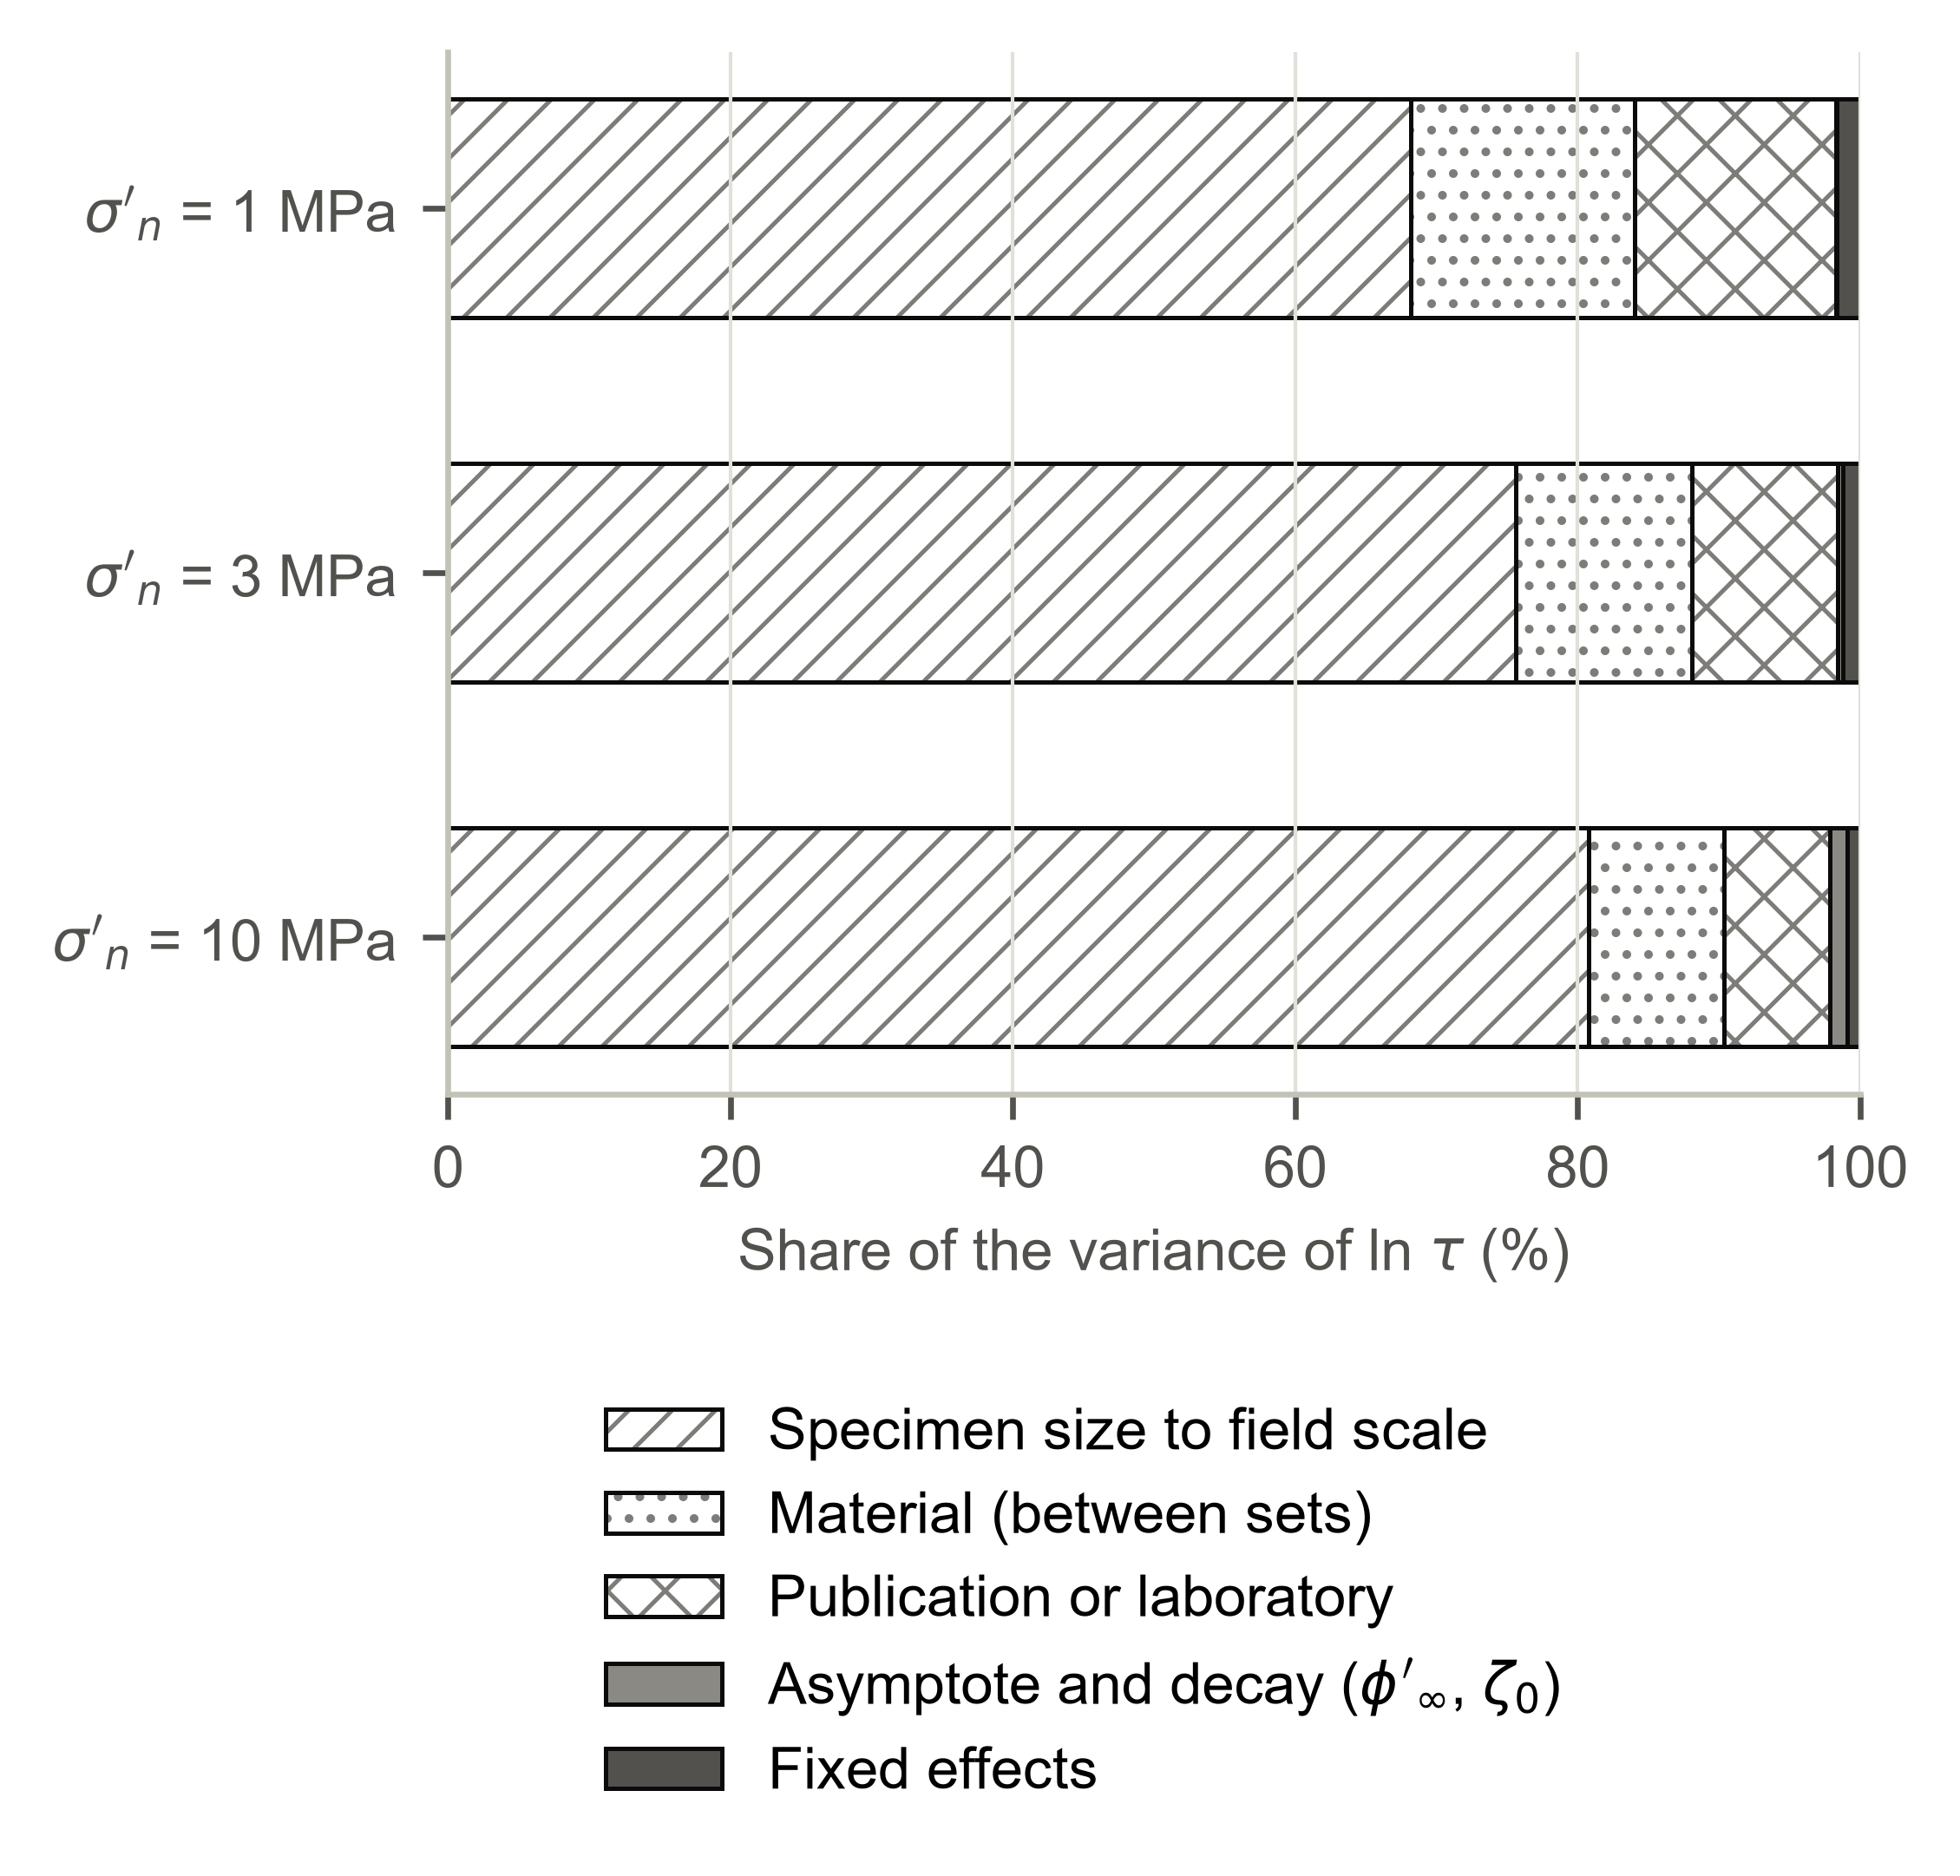
\includegraphics[width=3.5in]{FigS5_variance.png}
\caption{Shares of the variance of the mean-envelope ln $\tau$ for an untested material of low rock quality placed at e = 0.65, scaled from 100 mm to 1 m maximum particle size, at three normal stresses.}
\end{figure}
\clearpage
\begin{table}[htbp]
\caption{Mode B: every procedure evaluated (held-out tests at $\sigma'_n$ $\ge$ 2 MPa predicted from tests at $\sigma'_n$ $\le$ 1.5 MPa of the same set)}
\centering\footnotesize
\renewcommand{\arraystretch}{1.2}
\setlength{\tabcolsep}{3.5pt}
\begin{tabular}{p{1.7in}ccccccc}
\hline
Procedure & 80\% coverage & Below P05 & Below P10 & Mean z & CRPS & $\Delta$ CRPS & Holm p \\
\hline
Prior, no site tests & 88\% & 4\% & 12\% & $-$0.20 & 0.0455 & +0.0097 & 1.00 \\
Least-squares fit of $\phi'_1$, m = 0.90 & 82\% & 6\% & 18\% & $-$0.77 & 0.0433 & +0.0075 & 1.00 \\
Least-squares fit of $\phi'_1$, m from training data & 84\% & 2\% & 6\% & +0.13 & 0.0305 & $-$0.0053 & 1.00 \\
Joint update of both random effects & 76\% & 14\% & 24\% & $-$0.64 & 0.0333 & $-$0.0025 & 0.75 \\
Level update of each set (Eq. 8) & 80\% & 14\% & 20\% & $-$0.56 & 0.0358 & --- & --- \\
Level update, flagged sets discarded & 80\% & 12\% & 20\% & $-$0.54 & 0.0361 & +0.0003 & 1.00 \\
Flagged sets discarded, shared laboratory effect & 74\% & 14\% & 26\% & $-$0.62 & 0.0386 & +0.0028 & 1.00 \\
\hline
\end{tabular}
\par\vspace{4pt}\parbox{\linewidth}{\footnotesize Note: 50 held-out tests at $\sigma'_n$ $\ge$ 2 MPa on 39 sets from 6 laboratories (11 publications), predicted from tests at $\sigma'_n$ $\le$ 1.5 MPa of the same set. Mean z: mean standardized residual (negative: strength overpredicted). The procedures were developed while examining earlier versions of the model on related held-out sets, so the comparisons are exploratory. p-values from exact sign-flip tests on laboratory means, Holm-adjusted within Mode B. CRPS in units of ln $\tau$; $\Delta$ CRPS relative to the level update. In the design procedure, the lower of the level-updated and prior percentiles is used above the largest $\sigma'_n$ of the site tests.}
\end{table}
\begin{table}[htbp]
\caption{Secant friction angle $\phi'_s$ (\textdegree{}) of the waste rock of the example, median / 5th percentile of the mean envelope}
\centering\small
\renewcommand{\arraystretch}{1.2}
\setlength{\tabcolsep}{3.5pt}
\begin{tabular}{lccc}
\hline
Material & Laboratory, 1 MPa & Placed, 1 MPa & Placed, 2 MPa \\
\hline
Rock type A & 41.9 / 37.7 & 37.2 / 30.5 & 35.5 / 29.4 \\
Rock type B & 43.5 / 39.1 & 38.9 / 32.0 & 36.8 / 30.4 \\
Rock type C & 40.6 / 36.4 & 37.0 / 29.7 & 35.4 / 28.5 \\
Rock type D (untested) & 41.5 / 37.3 & 37.1 / 30.1 & 35.5 / 29.0 \\
Rock type E (untested) & 41.5 / 37.3 & 35.1 / 28.3 & 33.8 / 27.5 \\
Dump average, model correlation & 42.0 / 39.3 & 37.4 / 31.3 & 35.7 / 29.8 \\
Dump average, full correlation & 42.0 / 37.7 & 37.4 / 30.5 & 35.7 / 29.2 \\
\hline
\end{tabular}
\par\vspace{4pt}\parbox{\linewidth}{\footnotesize Note: Laboratory: specimen void ratio and size. Placed: void ratio 0.65 (rock type E, 0.80), maximum particle size 1 m, size effect with zero mean. Each rock type is represented by a new set from the site laboratory. The full-correlation case sorts the samples of each rock type at every stress, an upper bound on dependence.}
\end{table}
\begin{table}[htbp]
\caption{Structural comparison of mean and covariance forms (data without censoring)}
\centering\footnotesize
\renewcommand{\arraystretch}{1.2}
\setlength{\tabcolsep}{3.5pt}
\begin{tabular}{llp{1.6in}ccc}
\hline
Model & Mean & Random-effect covariance & Parameters & Log-likelihood & Out-of-sample log score \\
\hline
M1 & Bounded & Stress-decreasing (gradient of the mean) & 17 & 956.7 & 946.8 \\
M2 & Bounded & Additive (level and slope) & 17 & 953.5 & 943.9 \\
M4b & Quadratic by class & Stress-decreasing (from M1) & 17 & 953.0 & 940.5 \\
M3b & Quadratic by class & Additive & 17 & 949.6 & 937.4 \\
M4 & Quadratic & Stress-decreasing (from M1) & 15 & 945.5 & 935.7 \\
M3 & Quadratic & Additive & 15 & 940.9 & 931.2 \\
\hline
\end{tabular}
\par\vspace{4pt}\parbox{\linewidth}{\footnotesize Note: 741 tests without censoring or truncation; all models include rock quality class, void ratio, and ln Dmax. Log-likelihood: maximum likelihood with the exact Gaussian marginal for each publication, given the covariance structure; for M1 and M2, maximum over $\phi'_\infty$ from 20\textdegree{} to 28\textdegree{}. Out-of-sample: joint log score leaving out one publication at a time with the variance parameters fixed. First-order minus Laplace log-likelihood of M1: 1.1 at 20\textdegree{}, 1.8 at 22\textdegree{}, 3.0 at 24\textdegree{}, 3.9 at 25\textdegree{}, 3.8 at 26\textdegree{}, 9.9 at 28\textdegree{}; the Laplace maximum was 954.2. Largest single-publication contribution to M1 $-$ M3: 7.2 of 15.8.}
\end{table}
\begin{table}[htbp]
\caption{Mode A with censored tests: fractions below the 5th and 10th percentiles}
\centering\footnotesize
\renewcommand{\arraystretch}{1.2}
\setlength{\tabcolsep}{3.5pt}
\begin{tabular}{lccc}
\hline
Band and form & Below P05 & Below P10 & Mean z \\
\hline
All stresses (741 tests, 55 censored, 23 laboratories) &  &  &  \\
   HiBER, bounded & 4.9\%--5.8\% & 8.4\%--9.7\% & +0.06 \\
   HiBER, quadratic & 4.7\%--5.4\% & 7.2\%--8.2\% & +0.09 \\
   HiBER, power & 4.6\%--5.3\% & 7.0\%--8.1\% & +0.11 \\
   Leps 2.0, hierarchical dispersion & 3.4\%--3.6\% & 4.5\%--5.0\% & +0.31 \\
   Leps 2.0, constant dispersion & 4.0\%--4.5\% & 5.7\%--6.2\% & +0.22 \\
$\sigma'_n$ $\ge$ 2 MPa (146 tests, 28 censored, 8 laboratories) &  &  &  \\
   HiBER, bounded & 6.8\%--7.5\% & 11.0\%--12.3\% & $-$0.05 \\
   HiBER, quadratic & 4.1\% & 5.5\% & +0.17 \\
   HiBER, power & 4.1\% & 5.5\% & +0.24 \\
   Leps 2.0, hierarchical dispersion & 4.8\% & 6.2\% & $-$0.09 \\
   Leps 2.0, constant dispersion & 4.1\% & 6.2\% & $-$0.26 \\
$\sigma'_n$ $\ge$ 3 MPa (90 tests, 24 censored, 5 laboratories) &  &  &  \\
   HiBER, bounded & 6.7\% & 7.8\% & +0.07 \\
   HiBER, quadratic & 3.3\% & 3.3\% & +0.24 \\
   HiBER, power & 3.3\% & 3.3\% & +0.33 \\
   Leps 2.0, hierarchical dispersion & 3.3\% & 4.4\% & $-$0.10 \\
   Leps 2.0, constant dispersion & 3.3\% & 4.4\% & $-$0.29 \\
\hline
\end{tabular}
\par\vspace{4pt}\parbox{\linewidth}{\footnotesize Note: Censored tests (axial strain at the maximum deviator $\ge$ 19\%) are lower bounds of strength. Ranges: lower value counts a censored test as below a percentile only if its lower bound is; upper value counts it always. Mean z: mean standardized residual of the uncensored tests. Nominal: 5\% and 10\%.}
\end{table}
\section*{Worked Example of the Update}
The example follows Eqs. (3)--(9) of the paper at the maximum-likelihood point of the ridge ($\phi'_\infty$ = 29\textdegree{}, $\zeta_0$ = 0.428), with the published parameters, and is checked against the implementation, which also averages over the ridge and the posterior of the variance parameters. Material: low rock quality, specimen void ratio 0.35, maximum particle size 178 mm; placement void ratio 0.65 and field size 1 m.

\paragraph{Step 1: Site tests.}
Three drained tests at $\sigma'_3$ = 0.3, 0.7, 1.2 MPa failed at $\sigma'$1 = 1.71, 3.42, 5.34 MPa. With the conversion of Cylwik et al. (2025) and m = 0.883 (the local slope of the prior at 1 MPa), they give $\sigma'_n$ = 0.544, 1.228, 2.060 MPa and $\tau$ = 0.534, 1.076, 1.679 MPa, that is, x = -0.622, 0.192, 0.710 and y = -0.640, 0.060, 0.505.

\paragraph{Step 2: Conflict check.}
The prior mean at the tests is f = -0.673, 0.039, 0.500, the residuals are r = 0.032, 0.021, 0.005, and $\sigma_\varepsilon$ = 0.041, 0.035, 0.031. With V from Eq. (7) built with the matrices below, D$^{2}$ = 0.15 with 3 degrees of freedom (p = 0.986): no conflict.

\paragraph{Step 3: Cut update.}
At the centroid $\bar{x}$ = 0.093, the gradient a stacks the gradient of the envelope with respect to ($\eta$, $\zeta$) for the laboratory and the set effects and with respect to the fixed effects; $g_0=\mathbf{a}^T\mathbf{P}\mathbf{a}$ = 0.0116. Eq. (8) gives $\hat q_0$ = 0.0167 with variance 0.00040. The shift $\mathbf{P}\mathbf{a}\hat q_0/g_0$ raises $\eta$ by 0.0076 through the laboratory effect and by 0.0085 through the set effect, and moves the fixed effects slightly.

\paragraph{Step 4: Rock type, density, and size.}
The rock type is represented by a new set from the same laboratory: the updated laboratory and fixed effects are kept, and the set effect is drawn again from $\mathbf{G}_s$. The void ratio is then changed to the placement value through $\eta$, and the size shift adds a variance of (ln(D\_f/D\_l))$^{2}$(SE$^{2}$ + $\tau_D^{2}$) with zero mean. Above the largest $\sigma'_n$ of the tests (2.06 MPa), the lower of the updated and prior percentiles is used.
\begin{table}[htbp]
\caption{Worked example: secant friction angle $\phi'_s$ (\textdegree{}), median / 5th percentile of the mean envelope}
\centering\footnotesize
\renewcommand{\arraystretch}{1.2}
\setlength{\tabcolsep}{3.5pt}
\begin{tabular}{lcccc}
\hline
Stage & 0.5 MPa & 1 MPa & 3 MPa & 5 MPa \\
\hline
Prior, laboratory & 43.9 / 38.2 & 41.3 / 36.3 & 38.0 / 33.5 & 36.7 / 32.4 \\
Updated (rock type), laboratory & 44.1 / 39.1 & 41.6 / 37.2 & 38.2 / 34.1 & 36.9 / 32.9 \\
Prior, placed and field size & 39.1 / 31.3 & 37.2 / 30.1 & 34.9 / 28.4 & 34.0 / 27.8 \\
Updated (rock type), placed and field size & 39.3 / 32.0 & 37.4 / 30.6 & 35.1 / 28.8 & 34.2 / 28.1 \\
Design 5th percentile & 32.0 & 30.6 & 28.4 & 27.8 \\
Implementation (envolvente\_diseno) & 39.3 / 32.0 & 37.4 / 30.6 & 34.8 / 28.4 & 33.9 / 27.7 \\
\hline
\end{tabular}
\par\vspace{4pt}\parbox{\linewidth}{\footnotesize Note: Plug-in values at the maximum-likelihood point; the implementation averages over the ridge of ($\phi'_\infty$, $\zeta_0$) and the posterior of the variance parameters (conflict p = 0.984).}
\end{table}
\paragraph{Published matrices.}
Fixed effects $\beta$ = (0.2036, 0.0872, 0.0280, $-$0.4879, 0.0216, $-$0.0675, $-$0.1005) in the order of Table 1 ($\beta_c$ good, moderate, low; $\beta_e$; $\kappa$; $\delta$\_c moderate, low). Dispersion: ln $\sigma_\varepsilon$ = -3.316 $-$0.207x.
\begin{center}\footnotesize
\textbf{Covariance of the fixed effects, $\mathbf{C}_\beta \times 10^4$}\\[2pt]
\begin{tabular}{lrrrrrrr}
\hline
 & $\beta$ good & $\beta$ moderate & $\beta$ low & $\beta_e$ & $\kappa$ & $\delta$ moderate & $\delta$ low \\
\hline
$\beta$ good & 12.07 & 7.58 & 5.23 & $-$12.28 & 0.39 & 0.04 & 0.17 \\
$\beta$ moderate & 7.58 & 8.71 & 4.65 & $-$10.58 & 0.27 & $-$0.77 & 0.09 \\
$\beta$ low & 5.23 & 4.65 & 6.42 & $-$7.51 & 0.46 & 0.05 & $-$1.06 \\
$\beta_e$ & $-$12.28 & $-$10.58 & $-$7.51 & 23.23 & 0.39 & 0.01 & $-$0.12 \\
$\kappa$ & 0.39 & 0.27 & 0.46 & 0.39 & 0.75 & 0.04 & 0.00 \\
$\delta$ moderate & 0.04 & $-$0.77 & 0.05 & 0.01 & 0.04 & 5.00 & 0.75 \\
$\delta$ low & 0.17 & 0.09 & $-$1.06 & $-$0.12 & 0.00 & 0.75 & 5.92 \\
\hline
\end{tabular}
\\[8pt]\textbf{$\mathbf{G}_p$ and $\mathbf{G}_s$ (rows and columns $\eta$, $\zeta$), $\times 10^4$}\\[2pt]
\begin{tabular}{lrrrr}
\hline
 & $\eta$ (laboratory) & $\zeta$ (laboratory) & $\eta$ (set) & $\zeta$ (set) \\
\hline
$\eta$ & 53.65 & $-$4.68 & 59.56 & $-$20.21 \\
$\zeta$ & $-$4.68 & 61.64 & $-$20.21 & 78.26 \\
\hline
\end{tabular}
\end{center}
\setcounter{table}{5}
\begin{table}[htbp]
\caption{Factor of safety of dumps on a competent level foundation (Morgenstern--Price, Slide2), placed waste rock: median / 5th-percentile envelope}
\centering\small
\renewcommand{\arraystretch}{1.2}
\setlength{\tabcolsep}{3.5pt}
\begin{tabular}{lccc}
\hline
Envelope & 150 m & 400 m & 700 m \\
\hline
Dump average, model correlation & 1.80 / 1.40 & 1.62 / 1.28 & 1.54 / 1.22 \\
Dump average, full correlation & 1.79 / 1.34 & 1.61 / 1.24 & 1.53 / 1.19 \\
Weakest tested rock type only & 1.76 / 1.29 & 1.59 / 1.20 & 1.52 / 1.15 \\
Untested, degraded rock type E only & 1.62 / 1.20 & 1.49 / 1.14 & 1.43 / 1.10 \\
\hline
\end{tabular}
\par\vspace{4pt}\parbox{\linewidth}{\footnotesize Note: Uniform dry face without benches; unit weight 17.2 kN/m\textsuperscript{3} (rock type E only: 15.7 kN/m\textsuperscript{3}). Monte Carlo at 700 m with 600 envelope samples, each with its own search: model correlation 0 failures (lognormal reliability index 3.2); rock type E only 5 (index 2.3). 700 m, model correlation: without size shift 1.54 / 1.40; laboratory density with size shift (21 kN/m\textsuperscript{3}) 1.74 / 1.38; laboratory density and size 1.74 / 1.59; size effect at its estimated mean 1.62 / 1.29; Weibull scaling 1.40 / 1.12; independent size shifts per rock type 1.55 / 1.35; tested samples taken as representative 1.51 / 1.22; quadratic form 1.49 / 1.19.}
\end{table}
\end{document}
